\documentclass{beamer}
%\documentclass[handout]{beamer}

%\setbeamertemplate{background canvas}[vertical shading][bottom=white,top=structure.fg!25]
% or whatever

\usetheme[compress]{Amsterdam}
%\setbeamertemplate{headline}{}
%\setbeamertemplate{footline}{}
%\setbeamersize{text margin left=0.5cm}
  
\usepackage[english]{babel}
\usepackage{listings}
\usepackage{geometry}
\usepackage{hyperref}


\usepackage[utf8]{inputenc}
\usepackage[T1]{fontenc}
\usepackage{lmodern}

\lstset{
basicstyle=\scriptsize\ttfamily,
columns=flexible,
breaklines=true,
numbers=left,
%stepsize=1,
numberstyle=\tiny,
backgroundcolor=\color[rgb]{0.85,0.90,1}
}


\begin{document}

\title[Big Data and Automated Content Analysis]{\textbf{Big Data and Automated Content Analysis I+II} \\ Week 1 -- Wednesday \\ »Introduction«}
\author[Damian Trilling]{Damian Trilling \\ ~ \\ \footnotesize{d.c.trilling@uva.nl \\@damian0604} \\ \url{www.damiantrilling.net}}
\date{5 February 2019}
\institute[UvA]{Afdeling Communicatiewetenschap \\Universiteit van Amsterdam}


\begin{frame}{}
\titlepage
\end{frame}

\begin{frame}{Today}
\tableofcontents
\end{frame}



\section{Introducing\ldots}
\subsection{\ldots the people}

\begin{frame}
	Introducing\ldots \\
	~~~~~~~~\ldots the people
\end{frame}

\begin{frame}{Introducing\ldots}
	{\huge{Damian}}
	\small{}
	\begin{columns}
		\column{.3\textwidth}
		\makebox[\columnwidth]{
			\includegraphics[width=\columnwidth,height=\paperheight,keepaspectratio]{../../pictures/damian.jpg}}
		\column{.7\textwidth}
		dr. Damian Trilling \\
		Assistant Professor Political Communication \& Journalism \\
		\begin{itemize}
			\item studied Communication Science in M\"unster and at the VU 2003--2009
			\item PhD candidate @ ASCoR 2009--2012
			%\item now: Universitair Docent (UD) / Assistant Professor
			\item interested in political communication and journalism in a changing media environment and in innovative (digital, large-scale, computational) research methods
		\end{itemize}
		@damian0604 ~~ d.c.trilling@uva.nl ~~ REC-C~8\textsuperscript{th}~floor ~~ \url{www.damiantrilling.net} 
	\end{columns}
\end{frame}

\begin{frame}{Introducing\ldots} {\huge{Anne}} \small{} 
	\begin{columns}[] \column{.3\textwidth} \makebox[\columnwidth]{ \includegraphics[width=\columnwidth,height=\paperheight,keepaspectratio]{../../pictures/anne.jpg}} \column{.7\textwidth} dr. Anne Kroon \\ 
Assistant Professor Corporate Communication
 \begin{itemize} 
 	\item Stereotypes in the media
 	\item ACA and word embeddings
 \end{itemize} @annekroon ~~ a.c.kroon@uva.nl \end{columns} \end{frame}



\begin{frame}{Introducing\ldots}
	{\huge{You}}
	\small{}
	\begin{columns}
		\column{.3\textwidth}
		\makebox[\columnwidth]{
			\includegraphics[width=\columnwidth,height=\paperheight,keepaspectratio]{../../pictures/mannetje.png}}
		\column{.7\textwidth}
		Your name?\\
		Your background?\\
		Your reason to follow this course?
	\end{columns}
\end{frame}





\section{What is Big Data?}
\subsection{Definitions}

\begin{frame}
What is Big Data?
\end{frame}


{\setbeamercolor{background canvas}{bg=black}
\begin{frame}[plain]
\makebox[\linewidth]{
\includegraphics[width=\paperwidth,height=\paperheight,keepaspectratio]{../../pictures/bigdataisliketeenagesex.jpg}
}
\end{frame}
}


%\begin{frame}{What is Big Data?}
%What would \emph{you} call Big Data?
%\end{frame}

\begin{frame}{What is Big Data?}
\begin{block}{A simple technical definition could be:}<2->
Everything that needs so much computational power and/or storage that you cannot do it on a regular computer.
\end{block}
\end{frame}

\begin{frame}{What is Big Data?}
\begin{block}{Vis, 2013}<2->
\begin{itemize}
\item<2,4> ``commercial'' definition (Gartner): ``'Big data' is high-volume, -velocity and -variety information assets that demand cost-effective, innovative forms of information processing for enhanced insight and decision making''
\item<3-> boyd \& Crawford definition: 
\begin{enumerate}
\item Technology: maximizing computation power and algorithmic accuracy to gather, analyze, link, and compare large data sets.
\item Analysis: drawing on large data sets to identify patterns in order to make economic, social, technical, and legal claims.
\item Mythology: the widespread belief that large data sets offer a higher form of intelligence and knowledge that can generate insights that were previously impossible, with the aura of truth, objectivity, and accuracy.
\end{enumerate}
\end{itemize}
\end{block}
\end{frame}


\begin{frame}{Implications \& criticism}
\begin{block}{boyd \& Crawford, 2012}<2->
\begin{enumerate}
\item Big Data changes the definition of knowledge
\item Claims to objectivity and accuracy are misleading
\item Bigger data are not always better data
\item Taken out of context, Big Data loses its meaning
\item Just because it is accessible does not make it ethical
\item Limited access to Big Data creates new digital divides
\end{enumerate}
\end{block}
\end{frame}


\begin{frame}{APIs, researchers and tools \emph{make} Big Data}
\begin{block}{Vis, 2013}<2->
Inevitable influences of:
\begin{itemize}
\item APIs
\item filtering, search strings, \ldots
\item changing services over time
\item organizations that provide the data
\end{itemize}
\end{block}
\end{frame}
% vraag stellen: maar is dit anders dan met andere soorten onderzoek? Of is dit een principieel (wetenschapsfilosofisch?) probleem?


\begin{frame}{Epistemologies and paradigm shifts}
	\begin{block}{Kitchin, 2014}<1->
		\begin{itemize}
			\item<2-> (Reborn) empiricism: purely inductive, correlation is enough
			\item<3-> Data-driven science: knowledge discovery guided by theory
			\item<4-> Computational social science and digital humanities: employ Big Data research within existing epistemologies
			\begin{itemize}
				\item DH: descriptive statistics, visualizations
				\item CSS: prediction and simulation
			\end{itemize}
		\end{itemize}
	\end{block}
\end{frame}
% vraag stellen: maar is dit anders dan met andere soorten onderzoek? Of is dit een principiee




\subsection{Are we doing Big Data research?}

\begin{frame}{Are we doing Big Data research in this course?}
\begin{block}{Depends on the definition}<2->
\begin{itemize}
\item Not if we take a definition that \emph{only} focuses on computing power and the amount of data
\item<3-> \textbf{But:} We are using the same techniques. And they \emph{scale} well.
\item<4-> Oh, and about that high-performance computing in the cloud: We actually \emph{do} have access to that, so if someone has a really great idea\ldots
\end{itemize}

\end{block}
\end{frame}




\section{Methods}
\begin{frame}
Methods
\end{frame}

\subsection{Which techniques?}

\begin{frame}{What we will learn the next weeks}
\begin{block}{1. How to collect data}<2->
APIs, scrapers and crawlers, feeds, databases, \ldots \\
Storage in different file formats
\end{block}
\begin{block}{2. How to analyze data}<3->
Sentiment analysis, automated content analysis, regular expressions, natural language processing, cluster analysis,  machine learning, network analysis
\end{block}
\end{frame}


\begin{frame}{The ACA toolbox}
	\makebox[\columnwidth]{
		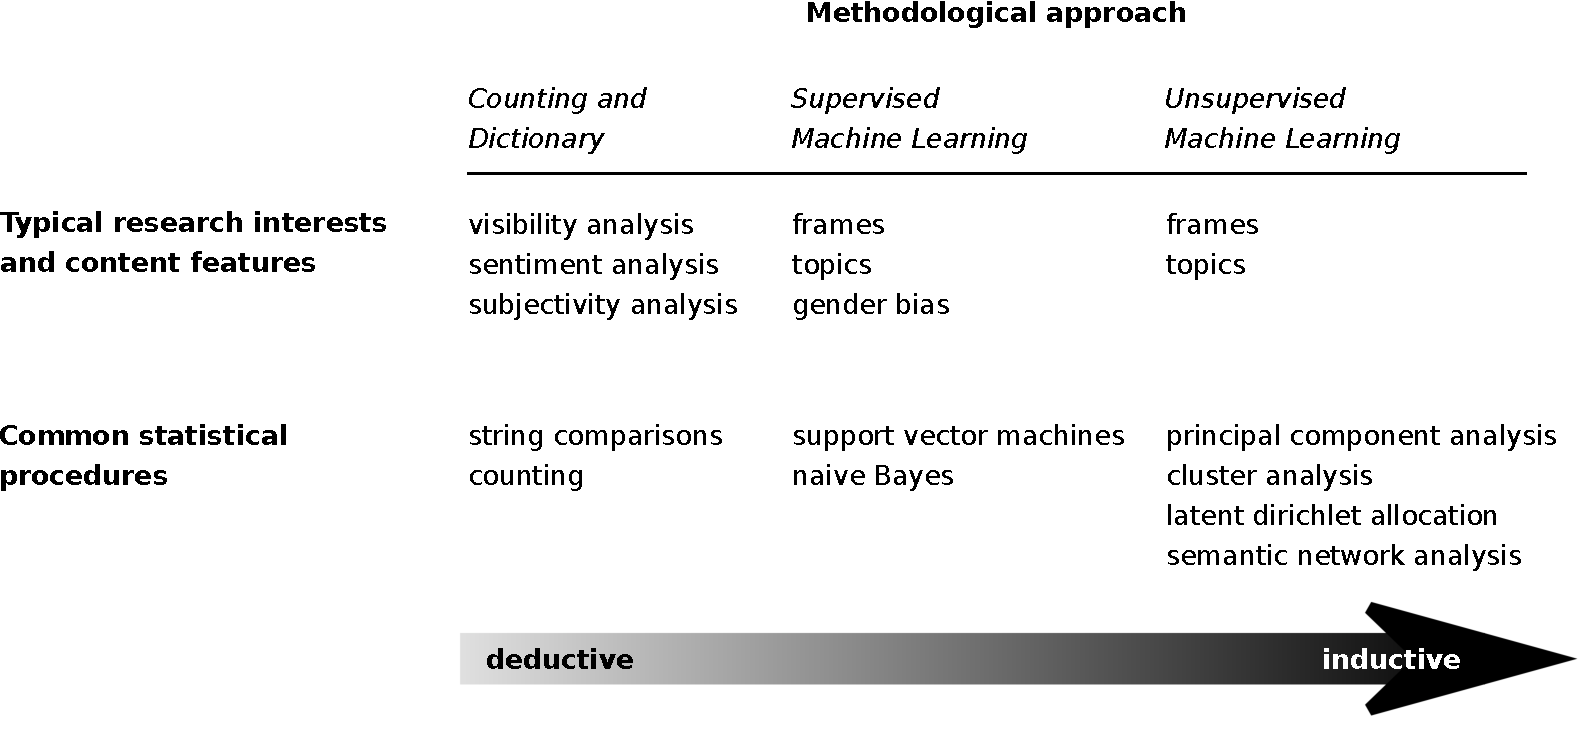
\includegraphics[width=\columnwidth,height=\paperheight,keepaspectratio]{../../pictures/boumanstrilling2016}}
	\\
	\tiny
	Boumans, J.W., \& Trilling, D. (2016). Taking stock of the toolkit: An overview of relevant automated content analysis approaches and techniques for digital journalism scholars. \emph{Digital Journalism, 4}, 1. 8--23.
\end{frame}


\subsection{Which tools?}


\begin{frame}{The methods}
\begin{block}{The tools we use for this}
The programming language Python (and the huge amount of Python modules others already wrote).
\end{block}
%\onslide<2->{But aren't there existing tools?}
%\onslide<3->{ --- sometimes. But look at this example:}
\end{frame}




\begin{frame}
	A language, not a program:\\
	\textbf{Python}
\end{frame}

\begin{frame}[plain]
\makebox[\columnwidth]{
	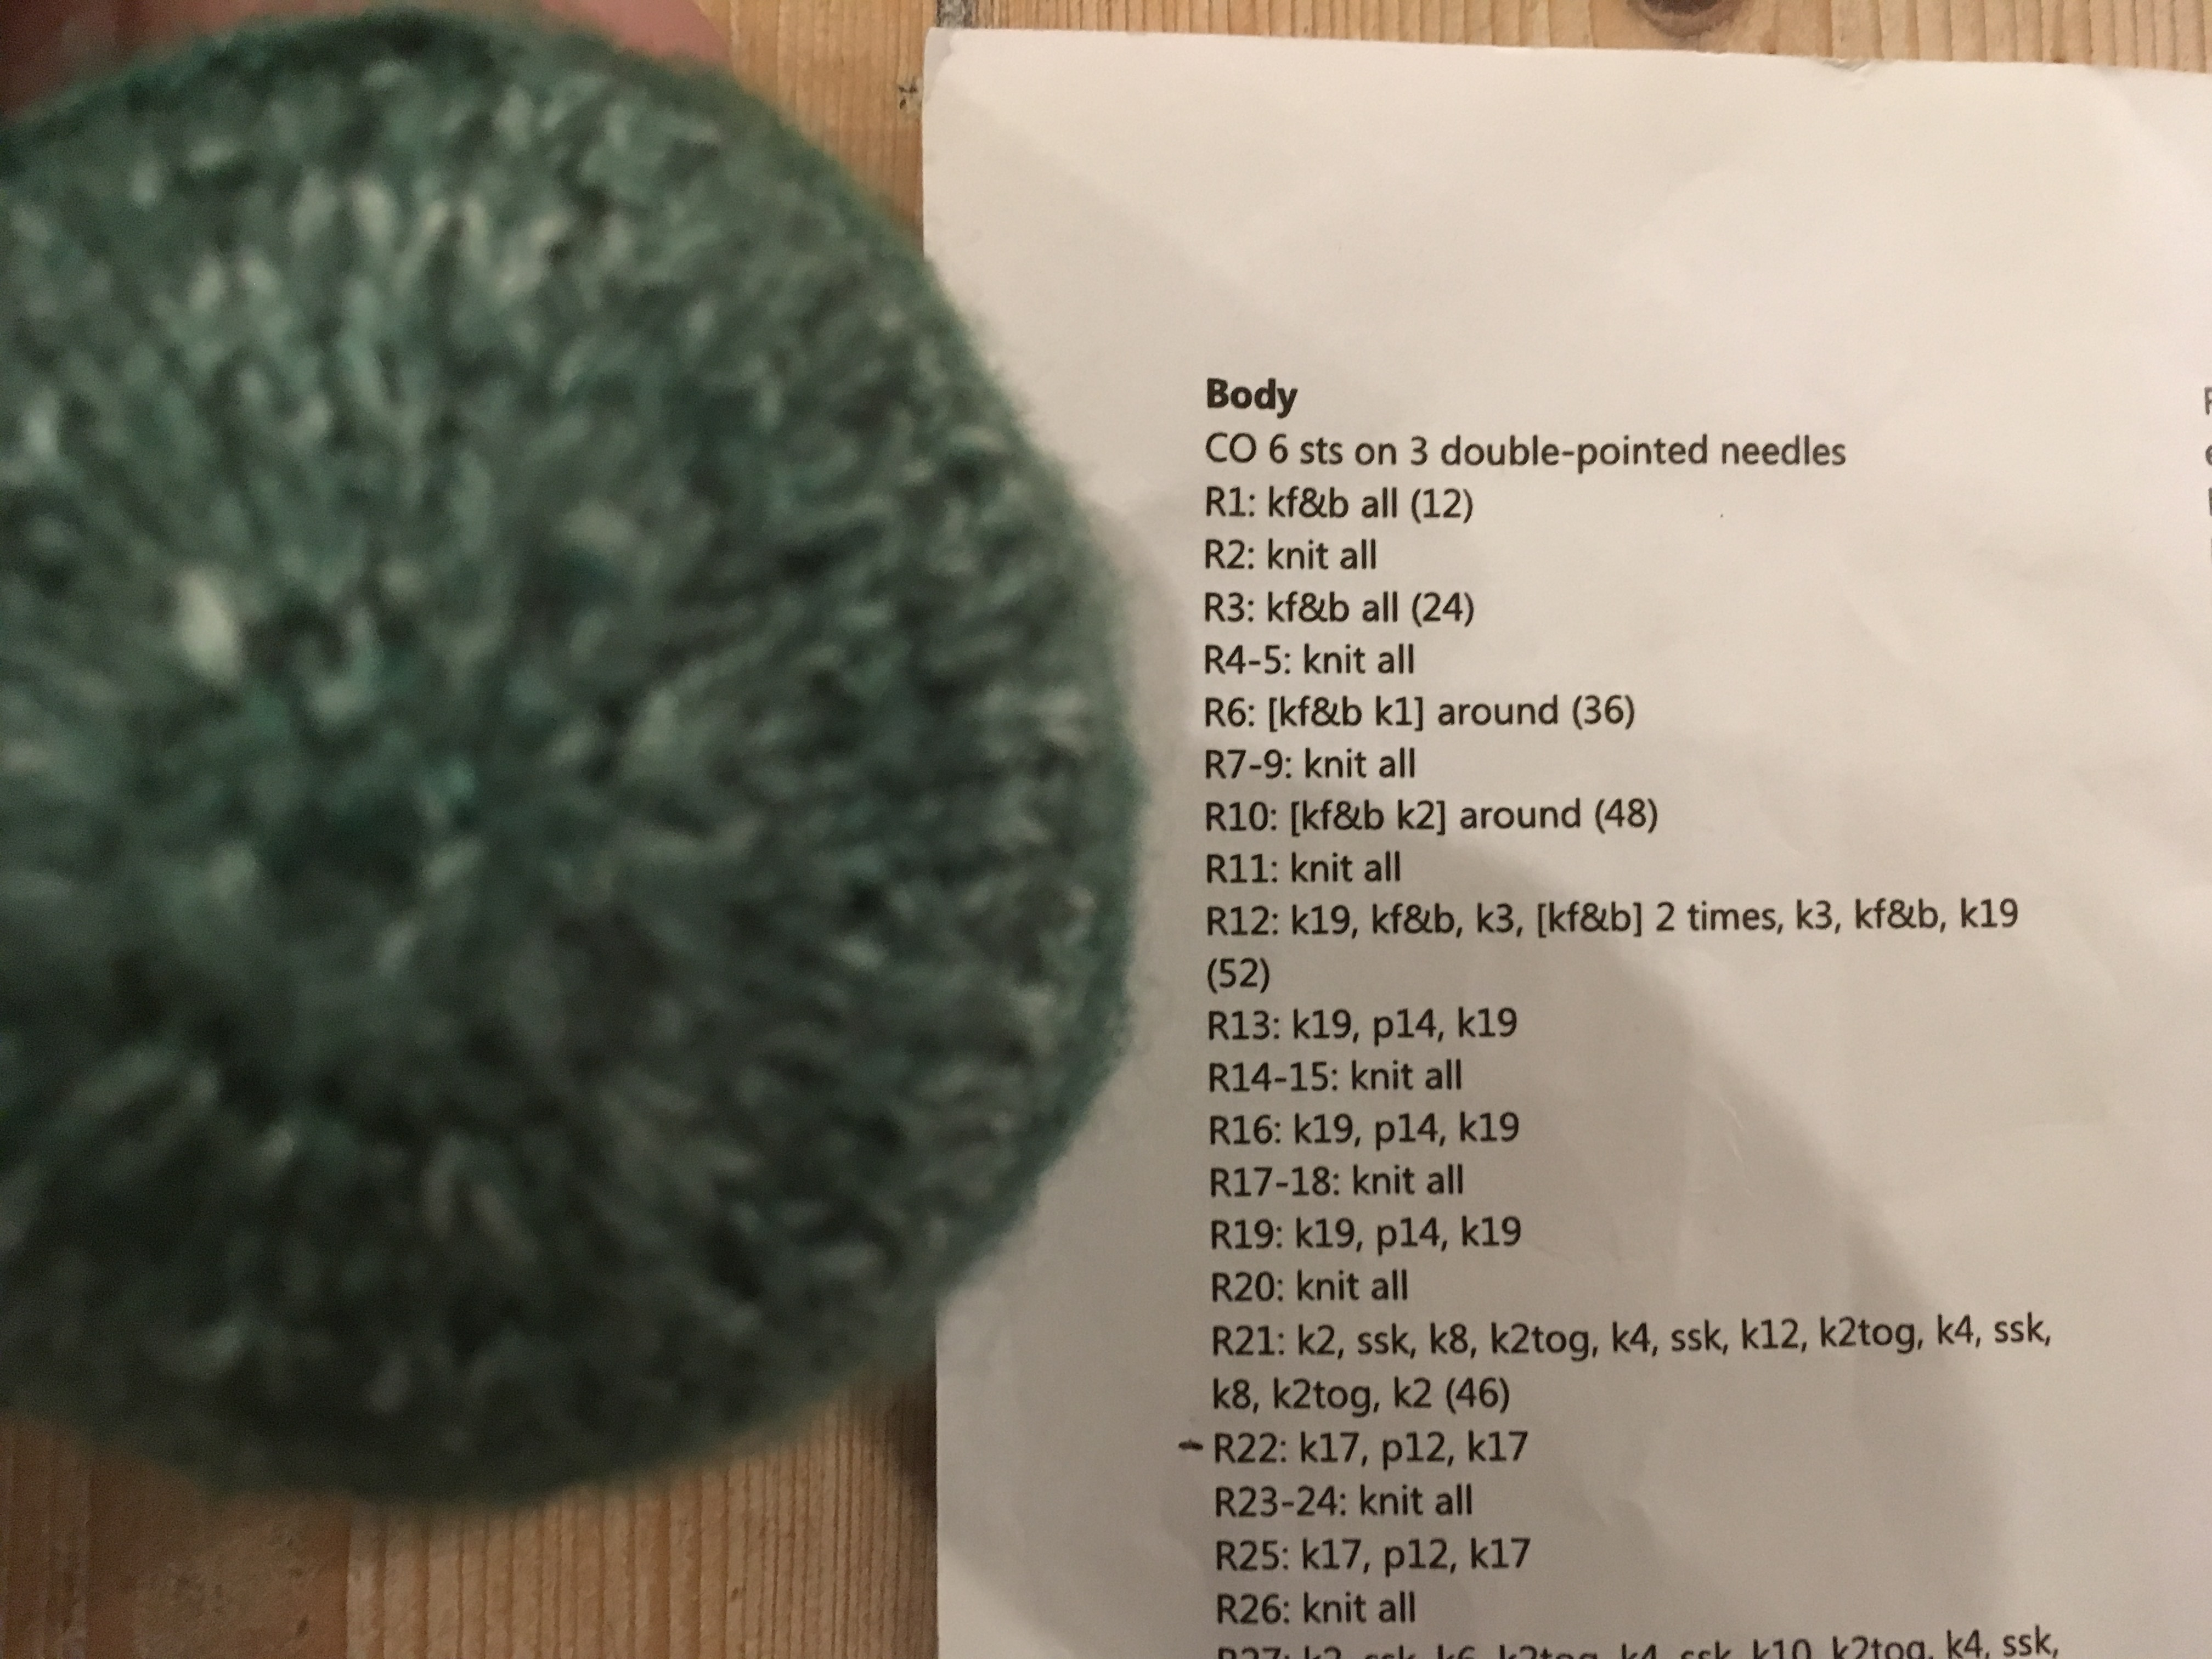
\includegraphics[width=\columnwidth,height=\paperheight,keepaspectratio]{../../pictures/knitting.jpg}}
\footnotesize{An algorithm in a language that's a bit harder (I think) than Python}
\end{frame}

\begin{frame}{Python}
	\begin{block}{What?}<1->
		\begin{itemize}
			\item A language, not a specific program
			\item Huge advantage: flexibility, portability
			\item One of \emph{the} languages for data analysis. \tiny{(The other one is R.)}
			\onslide<2>{ \\\tiny{But Python is more flexible---the original version of Dropbox was written in Python. Some people say: R for numbers, Python for text and messy stuff.}}
		\end{itemize}
	\end{block}
	
	\begin{block}{Which version?}<3->
		We use Python 3. \\ 
		\footnotesize{\url{http://www.google.com} or \url{http://www.stackexchange.com} still offer a lot of Python2-code, but that can easily be adapted. Most notable difference: In Python 2, you write {\tt print "Hi"}, this has changed to {\tt print ("Hi")}}\\
	\end{block}
\end{frame}

%
%
%\begin{frame}{If it's not a program, how do you work with it?}
%	\begin{block}{Interactive mode}<1->
%		\begin{itemize}
%			\item Just type {\tt python3} on the command line, and you can start entering Python commands {\tiny{(You can leave again by entering {\tt quit()})}}
%			\item Great for quick try-outs, but you cannot even save your code
%		\end{itemize}
%	\end{block}
%	
%	\begin{block}{An editor of your choice}<2->
%		\begin{itemize}
%			\item Write your program in any text editor, save it as {\tt myprog.py}
%			\item and run it from the command line with {\tt ./myprog.py} or {\tt python3 myprog.py}
%		\end{itemize}
%	\end{block}
%\end{frame}
%
%
%\begin{frame}{If it's not a program, how do you start it?}
%	\begin{block}{An IDE (Integrated Development Environment)}
%		\begin{itemize}
%			\item Provides an interface
%			\item Both quick interactive try-outs and writing larger programs
%			\item We use spyder, which looks a bit like RStudio (and to some extent like Stata)
%		\end{itemize}
%	\end{block}
%\end{frame}
%
%
%
%{\setbeamercolor{background canvas}{bg=black}
%	\begin{frame}[plain]
%		\makebox[\linewidth]{
%			\includegraphics[width=\paperwidth,height=\paperheight,keepaspectratio]{../../pictures/spyder-uitleg.png}
%		}
%	\end{frame}
%}
%
%



\begin{frame}{Why program your own tool?}
\makebox[\linewidth]{
\includegraphics[width=\paperwidth,height=.8\paperheight,keepaspectratio]{../../pictures/toolification.png}
}
\end{frame}

\begin{frame}{Why program your own tool?}
If the task would have been done with a (commercial) tool, we can only research what the tool allows us to do ($\Rightarrow$ our discussion from some minutes ago).
\begin{block}{Luckily, the problem is easily solved}<2->
The task was done with a self-written Python program. We change the line\\
\tt{~~~~lengte\_list.append(len(row\lbrack textcolumn\rbrack))}
\\ \normalfont{to}\\
\tt{~~~~lengte\_list.append(len(row\lbrack textcolumn\rbrack.split()))}
\end{block}
\end{frame}

\begin{frame}{Why program your own tool?}
\vspace{1cm}
{\tt \textbf
Moreover, the tools we use can limit the range of questions that might be imagined, simply because they do not fit the affordances of the tool. Not many researchers themselves have the ability or access to other researchers who can build the required tools in line with any preferred enquiry. This then introduces serious limitations in terms of the scope of research that can be done.}
\vspace{1cm}
\footnotesize{Vis, 2013\\}

\end{frame}


\begin{frame}{Why program your own tool?}
	\makebox[\linewidth]{
		\includegraphics[width=\paperwidth,height=.8\paperheight,keepaspectratio]{../../pictures/commercialpackages_anonymized.png}
	}
\end{frame}

\begin{frame}{Some considerations regarding the use of software in science}
Assuming that science should be \emph{transparent} and \emph{reproducible by anyone}\onslide<2->{, we should}
\begin{block}{use tools that are}<2->
\begin{itemize}
\item platform-independent 
\item free (as in beer and as in speech, gratis and libre)
\item which implies: open source
\end{itemize}
\end{block}
\onslide<3>{This ensures it can our research (a) can be reproduced by anyone, and that there is (b) no black box that no one can look inside. $\Rightarrow$ ongoing open-science debate!}
\end{frame}

\begin{frame}{Why program your own tool?}
\vspace{1cm}
{\tt \textbf
{[}\ldots{]} these {[}commercial{]} tools are often unsuitable for academic purposes because of their cost, along with the problematic ‘black box’ nature of many of these tools.}
{\footnotesize{Vis, 2013\\}}
\vspace{1cm}

{\tt \textbf
{[}\ldots{]} we should resist the temptation to let the opportunities and constraints of an application or platform determine the research question {[}\ldots{]}}
%\vspace{1cm}
{\footnotesize{Mahrt \& Scharkow, 2013, p. 30\\}}

\end{frame}



\section{What have others done?}
\begin{frame}
What have others done?
\end{frame}

\subsection{Online news sharing}
\begin{frame}{Online news sharing}
\begin{block}{The question}<2->
``We describe the interplay between website visitation patterns and social media reactions to news content. \lbrack\ldots\rbrack ~We also show  that social media reactions can help predict future visitation patterns early and accurately.'' (p.1)
\end{block}
\footnotesize{Castillo, El-Haddad, Pfeffer, \& Stempeck, 2013}
\end{frame}

\begin{frame}{Online news sharing}
\begin{block}{The method}
\begin{itemize}
\item data set 1: log files provided by Al Jazeera
\item data set 2: Facebook and Twitter API
\item analysis: link 1 and 2 and estimate the relationships  
\end{itemize}
\end{block}
\footnotesize{Castillo, El-Haddad, Pfeffer, \& Stempeck, 2013}
\end{frame}


{\setbeamercolor{background canvas}{bg=black}
\begin{frame}[plain]
\makebox[\linewidth]{
\includegraphics[width=\paperwidth,height=\paperheight,keepaspectratio]{../../pictures/castillo-ea-2014.png}
}
\end{frame}
}



\begin{frame}{Online news sharing}
\begin{block}{The issues}
\begin{itemize}
\item You need that guy at Al Jazeera
\item You need the infrastructure to cope with the data
\item Very much tailored to one outlet
\end{itemize}
\end{block}
\footnotesize{Castillo, El-Haddad, Pfeffer, \& Stempeck, 2013}
\end{frame}

\if true false
\subsection{Help requests on Facebook}
\begin{frame}{Help requests on Facebook}
\begin{block}{The question}<2->
Social Capital on SNS -- How do people request help on Facebook?
\end{block}
\footnotesize{Ellison, Gray, Vitak, Lampe, \& Fiore, 2013}
\end{frame}

\begin{frame}{Help requests on Facebook}
\begin{block}{The method}
\begin{itemize}
\item dataset: 20.000 ($n_{relevant} = 865$) Facebook status updates (access: via FB employee)
\item analysis: manual coding (field of action) and automated coding via LIWC (linguistic features)
\end{itemize}
\end{block}
\footnotesize{Ellison, Gray, Vitak, Lampe, \& Fiore, 2013}
\end{frame}

\begin{frame}{Help requests on Facebook}
\begin{block}{The issues}
\begin{itemize}
\item<2-> The bottleneck: low N due to need of human coders 
\item<3-> In that case: Additional value of automated linguistic coding?
\item<4-> Nobody uses public status messages -- bias?
\end{itemize}
\end{block}
\footnotesize{Ellison, Gray, Vitak, Lampe, \& Fiore, 2013}
\end{frame}
\fi



\subsection{Partisan asymmetries}
\begin{frame}{Partisan asymmetries}
\begin{block}{The question}<2->
How does the Twitter behavior differ between right-wing and left-wing users?
\end{block}
\footnotesize{Conover, Gonçalves, Flammini, \& Menczer, 2012}
\end{frame}

\begin{frame}{Partisan asymmetries}
\begin{block}{The method}
Starting with two hashtags (one used by progressives, one used by conservatives), 55 co-occuring hashtags were identified. Identification of follower networks, retweet networks, mention networks within tweets with these hashtags.
\end{block}
\footnotesize{Conover, Gonçalves, Flammini, \& Menczer, 2012}
\end{frame}



{\setbeamercolor{background canvas}{bg=black}
\begin{frame}[plain]
\makebox[\linewidth]{
\includegraphics[width=\paperwidth,height=\paperheight,keepaspectratio]{../../pictures/conover-ea-2012.png}
}
\end{frame}
}




\begin{frame}{Partisan asymmetries}
\begin{block}{The issues}
\begin{itemize}
\item The two seeds \#tcot and \#p2 oversample (extremly) partisan content, inevitably leading to the structure in Figure 3. 
\item But maybe no problem, as the rest of the paper aims to \emph{compare} these groups.
\item Not an empirical problem, but still: What do we learn \emph{exactly} from this study apart from the -- interesting -- case?
\end{itemize}
\end{block}
\footnotesize{Conover, Gonçalves, Flammini, \& Menczer, 2012}
\end{frame}




\section{What can we do?}

\subsection{Considerations regarding feasibility}
\begin{frame}{}
\huge{To which extent could \emph{we} conduct such studies?}
\end{frame}


\begin{frame}{What can we do?}
\begin{block}{Cool research, sure, but what can \emph{we} do?}
\begin{itemize}
\item Dependency from third parties: \\ scraping \textless ~ API \textless ~ server-side implementation 
\item Restrictions (e.g., Twitter: sprinkler, garden hose, fire hose) $\Rightarrow$ Vis, 2013: Data are made!
\item We can't just trust the numbers. Some tasks require human coders -- or a qualitative approach, at least as a pre-study.
\end{itemize}
\end{block}
\end{frame}


\begin{frame}{What can we do?}
\begin{block}{pros, cons, and feasibility}
\begin{itemize}
\item APIs (Twitter, Facebook, \dots)
\item server-side implementations ($\Rightarrow$ Al Jazeera-example)
\item scraping
\item client-side log files
\item "traditional" methods (surveys etc.)
\end{itemize}
\end{block}
\end{frame}

\begin{frame}{What can we do?}
\begin{block}{What helps us answer \emph{our} questions?}
\begin{enumerate}
\item Draft a RQ.
\item Think of \emph{different} ways to approach it
\item Think of \emph{different} data sources.
\item Think of \emph{different} analyses.
\end{enumerate}
\onslide<2->{
And then:
\begin{enumerate}
\item Check what the technical possibilities are. (e.g., is there an API? How can we get the data?)
\item Re-evaluate all steps.
\end{enumerate}
}
\end{block}
\end{frame}


\subsection{Examples from last year}
\begin{frame}{Some final projects from previous courses}
\begin{block}{Questions}
\begin{itemize}
%\item Are (popular) apps for children in the Apple App Store framed in terms of education or entertainment?
\item How can house prices on funda.nl be predicted?
\item Where are those who edit Wikipedia-entries about companies geographically located, related to the company's HQ?
%\item What are the sentiment and topical frames presented in Google US search results for the top political news search terms as indicated by Google Trends?
\item Can we predict ratings on Hostelworld?
\item What do people write in their Tinder profiles -- and how do men and women differ?
\item How international is the ICA, given all presentations given at all conferences in the last decade?
\end{itemize}
\end{block}

\end{frame}




\section{The schedule}
\begin{frame}
The schedule
\end{frame}

\begin{frame}{The schedule}
\begin{block}{Each week}
In general: A lecture (Wednesday) and a lab session (Friday). \\ Each week one method.
\end{block}
\begin{block}{Examinations}
A mid-term take-home exam in week 5 and an individual research project on which you work during the whole course.
\end{block}


\begin{alertblock}<2>{Self-study}
Play around! You really have to \emph{do} it to learn programming. See it as your weekly assignment ;-)
\end{alertblock}
\end{frame}


\subsection{Next meetings}
\begin{frame}
Next meetings
\end{frame}


\begin{frame}{Week 1: Introduction}

\begin{block}{Friday, 7--4}
No meeting due to \textit{Etmaal van de Communicatiewetenschap.}\\
\textbf{Your task: Read chapters 2 and 3! \\Test everything in your VM!}

\end{block}


\end{frame}
%
%\subsection{Preview}
%%\begin{frame}[plain]
%%	Let's start up Python and write a Hello-world-program!
%%\end{frame}
%
%
%
%
%\begin{frame}[fragile]{Start playing!}
%	Exercises 
%	
%	\vspace{.5cm}
%	\textbf{1. Run a program that greets you.}\\
%	The code for this is 
%	\begin{lstlisting}
%	print("Hello world")
%	\end{lstlisting}
%	After that, do some calculations. You can do that in a similar way:
%	\begin{lstlisting}
%	a=2
%	print(a*3)
%	\end{lstlisting}
%	Just play around.
%	
%	\vspace{.5cm}
%	\textbf{Additional ressources}\\
%	Codecademy course on Python
%	\url{https://www.codecademy.com/learn/python}
%
%\end{frame}
%



\end{document}


